\section{Results}

\medskip
\noindent\textit{Part 1: Does the separation happen, and what creates it?}

\subsection{What creates the separation}

We decompose the contribution of the two devices we add --- the horizon gate and the cross-covariance penalty --- by switching each on and off. The mechanism-free cell (Section~\ref{sec:xcov}) is also the baseline in which only the coordinate split remains.

\begin{table}[!tbp]
\caption{Separation index by mechanism. Cells are SEP (higher is better), $n=5$ seeds, $\lambda=4$. Bold marks the best cell in each row. The gate and the penalty are complementary: neither alone reaches what the two reach together.}
\label{tab:ablation}
\centering
\scriptsize
\begin{tabular}{llcccc}
\hline
Dataset & Stem & Neither & Gate only & xcov only & \textbf{Gate + xcov} \\
\hline
Synthetic & Reg & 0.135 & 0.342 & 0.279 & \textbf{0.408} \\
Synthetic & NCE & 0.121 & 0.124 & 0.488 & \textbf{0.749} \\
PTB-XL & Reg & 0.375 & 0.404 & 0.312 & \textbf{0.495} \\
PTB-XL & NCE & 0.392 & 0.503 & 0.283 & \textbf{0.567} \\
HAPT & Reg & 0.521 & 0.537 & 0.236 & \textbf{0.632} \\
HAPT & NCE & 0.297 & 0.366 & 0.162 & \textbf{0.515} \\
\hline
\end{tabular}
\end{table}

In Table~\ref{tab:ablation} the model with both devices ranks first in all six settings, and neither device alone reaches that value. On the contrastive stem of the synthetic data the gate alone is indistinguishable from the mechanism-free case (0.124 against 0.121), yet adding that same gate to the penalty raises SEP from 0.488 to 0.749: the two devices need each other. The penalty alone is actively harmful on the real data, breaking down the inclusion term and falling below even the mechanism-free case.

The ``Neither'' cells take the first 16 of the 64 dimensions, and their SEP agrees in all six settings to within 0.015 with the SEP of 16 dimensions drawn at random from the same embedding. Without our devices, any part of the embedding holds the two factors to a similar degree, so coordinate position carries no meaning by itself; our contribution is to give those coordinates structure.

\subsection{Separation requires a latent target}

This section ablates a third design axis, the \emph{target space}, testing the premise of the latent-prediction family: that prediction should be made in a latent space rather than on the raw signal. We hold the gate, the anchor, the horizon and the loss form fixed and change only what is predicted. The latent target is the 64-dimensional output the target encoder reads from the future interval; the raw target is the patch itself at that time (with one extra linear head). Both models carry the cross-covariance penalty, so $\lambda$ has the same meaning for each, and we compare each at its own best value over the swept curve.

\begin{table}[!tbp]
\caption{Latent target against raw target. Cells are SEP on synthetic, $n=5$ seeds, each stem at its own best $\lambda$. Bold marks the latent target. Everything but the prediction target is held fixed.}
\label{tab:latentraw}
\centering
\footnotesize
\begin{tabular}{lccc}
\hline
Stem & Latent (best) & Raw (best) & Difference \\
\hline
HGLP-Reg & \textbf{0.809} ($\lambda=1$) & 0.415 ($\lambda=4$) & $+0.394$ ($1.95\times$) \\
HGLP-NCE & \textbf{0.844} ($\lambda=16$) & 0.432 ($\lambda=16$) & $+0.411$ ($1.95\times$) \\
\hline
\end{tabular}
\end{table}



Replacing the latent target with raw patches halves SEP on both stems (Table~\ref{tab:latentraw}); since both carry the same penalty and are compared at their own optimal $\lambda$, neither side gains from the knob. The allocation term is the same for the two targets, at 0.86 to 0.89, and the gap opens in the inclusion term: the raw target loses the persistent factor as the penalty grows, falling from 0.807 to 0.401, whereas the latent target stays above 0.97 throughout. The raw signal still contains the transient component, and the pressure to predict it too pushes out the persistent factor. The gate and the penalty of Section~IV-A are thus not enough on their own; the latent target has to be present as well.

\subsection{Can post-hoc processing take its place?}

If an embedding trained without the gate is rotated post-hoc without labels --- by principal component analysis, by slowness-ordered independent component analysis, or by slow feature analysis (SFA) --- does it reach the same separation? These methods need no horizon gate at all, so they are the sharpest objection to our method.

\begin{table}[!tbp]
\caption{Our method against label-free post-hoc unmixings. Cells are SEP, $n=5$ seeds. Our method has one knob, so we report its best point on the swept $\lambda$ curve; each unmixing is a single fixed value. Bold marks the winner of each row. The verdict is three to three overall: two of two on synthetic, one of four on real data.}
\label{tab:rotation}
\centering
\scriptsize
\begin{tabular}{llccc}
\hline
Dataset & Stem & Ours (best $\lambda$) & SFA & Verdict \\
\hline
Synthetic & Reg & \textbf{0.814} ($\lambda=1$) & 0.446 & win \\
Synthetic & NCE & \textbf{0.849} ($\lambda=16$) & 0.388 & win \\
PTB-XL & Reg & 0.495 & \textbf{0.567} & loss \\
PTB-XL & NCE & 0.567 & \textbf{0.599} & loss \\
HAPT & Reg & 0.677 & \textbf{0.717} & loss \\
HAPT & NCE & \textbf{0.626} ($\lambda=64$) & 0.527 & win \\
\hline
\end{tabular}
\end{table}

\begin{figure*}[!tbp]
\centering
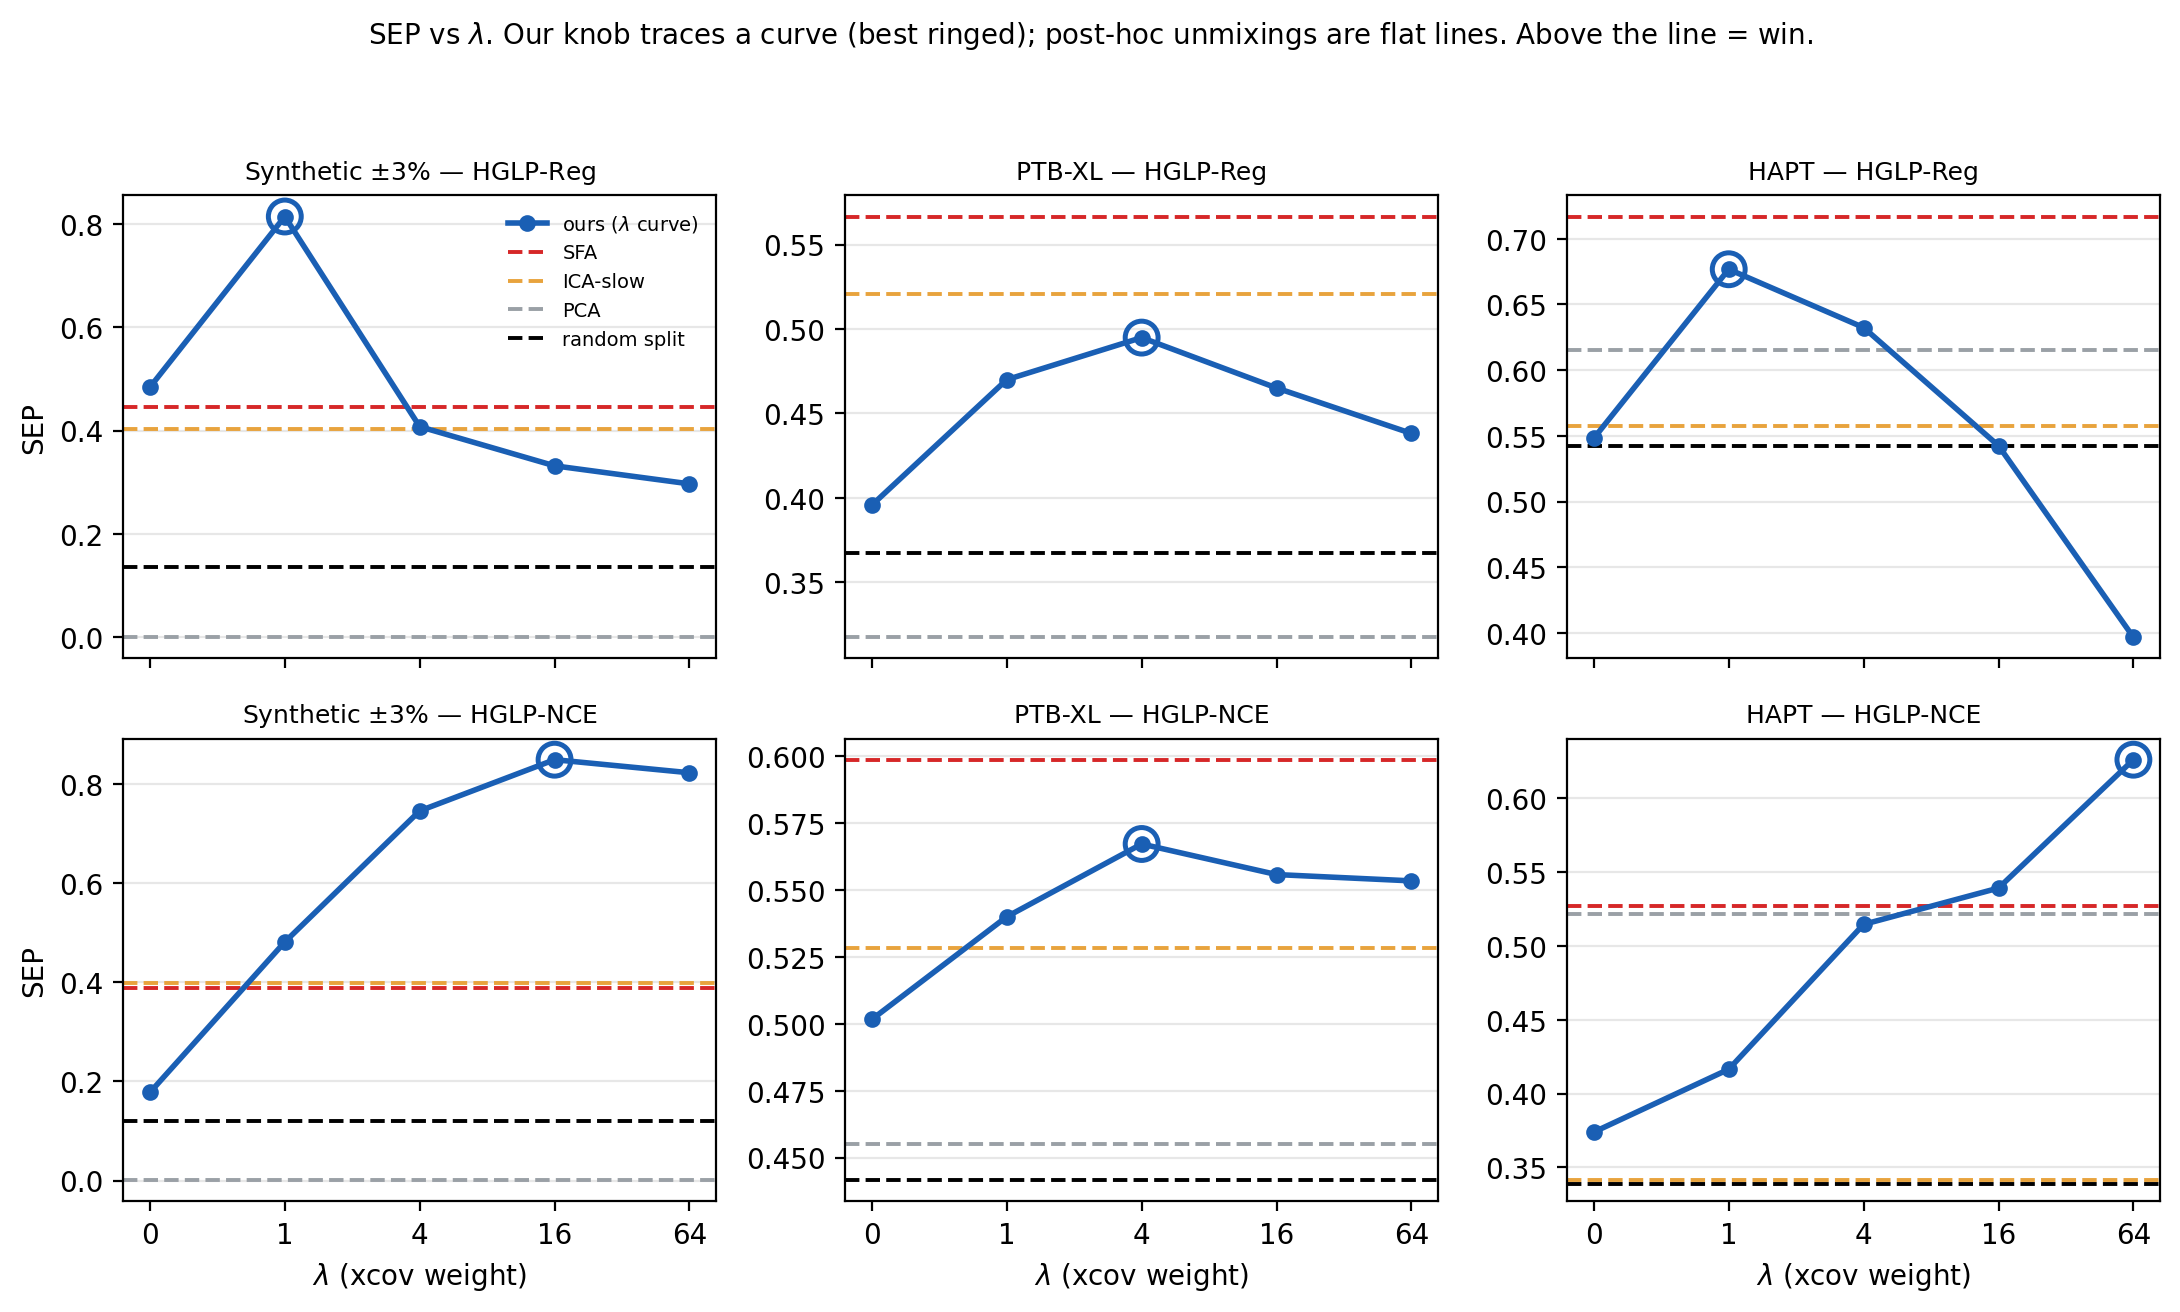
\includegraphics[width=0.70\textwidth]{figs/fig_rotation_sep.png}
\caption{SEP against the penalty weight $\lambda$. $n=5$ seeds. Our method traces a curve over $\lambda\in\{0,1,4,16,64\}$ with its best point ringed; each post-hoc unmixing has no knob and is a horizontal line. A win is our curve rising above the SFA line. Unlike an inclusion--exclusion plane, this view combines all three SEP terms, so it also shows the one real-data win, which the inclusion--exclusion plane cannot display.}
\label{fig:rotation}
\end{figure*}

We have one knob and the post-hoc rotations have none, so we report the whole curve rather than a single point (Table~\ref{tab:rotation}, Fig.~\ref{fig:rotation}); only our method has a knob that can be swept, and hiding that asymmetry would not make the comparison fair. On the synthetic data the curve passes above every post-hoc rotation point, and principal component analysis fails completely (SEP 0.000) --- direct evidence that a ranking by variance is not a ranking by persistence, since the transient factor crowds into the leading components and nothing is left in the complement. On the real data we do not lead: SFA reaches the same inclusion at a higher exclusion. The verdict over all six settings is three wins to three losses, but split apart it is two of two on synthetic and three losses of four on real data, with losing margins of 0.032 to 0.072 against a winning margin of 0.099.

This shortfall is expected. Persistence and spectral slowness coincide only under particular assumptions, and our synthetic data deliberately breaks that coincidence: the persistent factor hides inside the oscillation frequency and cannot be reached by low-pass filtering. On PTB-XL and HAPT the persistent factor largely coincides with the slow component, so SFA, which optimizes slowness directly, does the same job by a more direct route. Our advantage appears where the two axes come apart; where they coincide, post-hoc rotation already suffices. What remains ours is that the coordinates are fixed during training, so no second fitting stage is needed at deployment --- an operational difference, not a difference in the quality of the separation.

\medskip
\noindent\textit{Part 2: Practical effect and cost}

\subsection{The cost of separation, and stability under domain shift}

We measure two things: the downstream cost that accompanies the separation, and how far performance falls when a probe fitted with few labels is carried to a domain in which the transient factor has been perturbed. What we measure is not the difference in absolute performance between the two blocks but the difference in the drop each block suffers; a smaller drop for the gated block means the separation translates into stability under domain shift.



We measure the cost against the full embedding of a model trained with no mechanism at all rather than against our own $z_{\mathrm{full}}$, since the latter mixes in the effect of block width. Read that way, the cost is effectively zero on synthetic data and PTB-XL, and only HAPT shows a substantial value ($-0.111$ on the regression stem, $-0.072$ on the contrastive stem). HAPT is the only dataset in which the persistent factor is not constant within the window: 57\% of its windows straddle an activity transition.

The perturbed domain is made by multiplying the evaluation windows by a gain ($x \mapsto x\cdot(1+s)$, maximum perturbation $s=2$); this is a bijection and does not destroy the labels of the persistent factor --- even at maximum perturbation the HAPT activity labels survive at macro-F1 0.696 (chance 0.167). The encoder was trained on the clean domain alone, and the probe is fitted only on clean data with few labels (25 or 100); only the evaluation runs separately on clean and perturbed windows, so the probe never trains on the perturbation it is scored on.

\begin{table}[!tbp]
\caption{Degradation under domain shift: a difference of differences. Each cell is the drop in macro-F1 from the clean domain to the most perturbed one, for the gated block minus the same drop for a width-matched block of the mechanism-free model; paired by seed, $n=5$. Negative means the gated block degrades less. \textbf{These are differences of drops, not differences in absolute performance} --- the gated block does not overtake the mechanism-free one at any perturbation strength.}
\label{tab:shift}
\centering
\footnotesize
\begin{tabular}{lccc}
\hline
Setting & 25 labels & 100 labels & All labels \\
\hline
\textbf{HAPT / Reg} & $\mathbf{-0.113}\pm$\textbf{0.023} & $\mathbf{-0.096}\pm$\textbf{0.029} & $-0.053$$\pm$0.056 \\
HAPT / NCE & $-0.017$$\pm$0.072 & $+0.015$$\pm$0.012 & $+0.007$$\pm$0.016 \\
PTB-XL / Reg & $-0.044$$\pm$0.048 & $-0.033$$\pm$0.048 & $-0.024$$\pm$0.035 \\
PTB-XL / NCE & $-0.036$$\pm$0.032 & $-0.010$$\pm$0.024 & $-0.009$$\pm$0.024 \\
Synthetic / Reg & $-0.012$$\pm$0.102 & $+0.043$$\pm$0.099 & $+0.064$$\pm$0.077 \\
Synthetic / NCE & $-0.044$$\pm$0.069 & $-0.055$$\pm$0.054 & $-0.045$$\pm$0.055 \\
\hline
\end{tabular}
\end{table}

The downstream cost of the gated block is effectively zero on synthetic and PTB-XL and at most 0.11 macro-F1 on HAPT. On that same HAPT the gated block has the smallest drop under shift: at 25 labels its drop is 0.113 smaller than that of the width-matched mechanism-free block (Table~\ref{tab:shift}), five times the seed standard deviation. This is only a difference of drops. At no perturbation strength we tested does absolute performance overtake that model, and the effect exceeds the error bars in only one of the six settings, the HAPT regression stem; in the remaining five it lies within the noise, though by sign alone 17 of the 24 cells are negative.

The two results interlock: HAPT is both the dataset with the largest downstream cost and the only one with clear stability under domain shift, two sides of one phenomenon. The gate trades absolute performance for stability under domain shift; the two cannot be had together.

